\documentclass{zjumcm}
\usepackage[framed,numbered,autolinebreaks,useliterate]{mcode}

\newcommand\maketitlepage{
    \begin{titlepage} 
        \begin{center}
    
        \vspace{20mm}
        \zihao{-0}\heiti{浙江大学第十六届}\\[0.1cm]
        \zihao{-0}\heiti{大学生数学建模竞赛}\\[0.5cm]
        \zihao{3}{2018 年 5 月 2 日-5 月 12 日}\\[1cm]
        % \vspace{\fill}
    \setlength{\extrarowheight}{3mm}
    {\songti\zihao{2}	
    \begin{tabular}{rc}
        {\makebox[2\ccwd][s]{题目}}& \makebox[8em]{\songti A \ \ \ \ \  B}\\
        {\makebox[2\ccwd][s]{编号}}& \underline{\makebox[8em]{\songti 887}}\\
    \end{tabular}  
     }\\[2cm]

     \setlength{\extrarowheight}{0mm}
    {\songti\zihao{4}	
    \begin{tabular}{|p{1.8cm}|p{4.5cm}|p{4.5cm}|p{4.5cm}|}
        \hline
         & 参赛队员 1 & 参赛队员 1 & 参赛队员 1\\\hline
        \textbf{姓名} & & & \\\hline
        \textbf{学号} & & & \\\hline
        \textbf{院系} & & & \\\hline
        \textbf{专业} & & & \\\hline
        \textbf{手机} & & & \\\hline
        \textbf{Email} & & & \\\hline
    \end{tabular}  
     }\\[2cm]

    \vspace{\fill} 
    \zihao{2}\songti
    \textbf{浙江大学本科生院}\\
    \textbf{浙江大学数学建模实践基地}
    
    % 完整版实验报告请点击:\href{http://v.youku.com/}{完整实验报告} 
        \end{center}	
    \end{titlepage}
}
 
\graphicspath{{./pic/}} % 图片放在pic目录下

\begin{document}
\renewcommand\figurename{图} %使用中文图
\renewcommand\tablename{表} %使用中文表
\renewcommand{\contentsname}{目录} %使用中文目录
\renewcommand{\refname}{参考文献} %使用中文目录

    \maketitlepage
    \pagestyle{empty}

    \begin{abstract}{关键词1;关键词2}

        这里是摘要
    \end{abstract}
    \newpage
    \pagestyle{plain}

    \section{问题重述}

\subsection{问题背景}

插入表格:
\begin{table}[H]
    \centering
    \begin{tabular}{|p{1.8cm}|p{4.5cm}|p{4.5cm}|p{4.5cm}|}
        \hline
         & 参赛队员 1 & 参赛队员 1 & 参赛队员 1\\\hline
        \textbf{姓名} & & & \\\hline
        \textbf{学号} & & & \\\hline
        \textbf{院系} & & & \\\hline
        \textbf{专业} & & & \\\hline
        \textbf{手机} & & & \\\hline
        \textbf{Email} & & & \\\hline
    \end{tabular} 
    \caption{表格标题}\label{tab-1}
\end{table}

三线表:
\begin{table}[H]
    \centering
    \newcolumntype{F}{>{$}c<{$}}
    \begin{tabular}{FlF}
        \toprule  
         & \text{参数名称} & \text{参数取值}\\
        \midrule
        M & \text{小车质量} & \\
		m & \text{摆杆质量} & \\
		b & \text{小车摩擦系数} & \\
		l & \text{摆杆转动轴心到杆质心的长度} & \\
		I & \text{摆杆惯量} & \\
		F & \text{加在小车上的力} & \\
		x & \text{小车位置} & \\
		\phi & \text{摆杆与垂直向上方向的夹角} & \\
		\theta & \text{摆杆与垂直向下方向的夹角} & \\
        \bottomrule
    \end{tabular}
    \caption{各物理参数}\label{tab-arg}
\end{table}

插入图片,尽量使用H默认不浮动,图片引用使用ref指令,如图\ref{model}所示:
\begin{figure}[H]
	\centering
	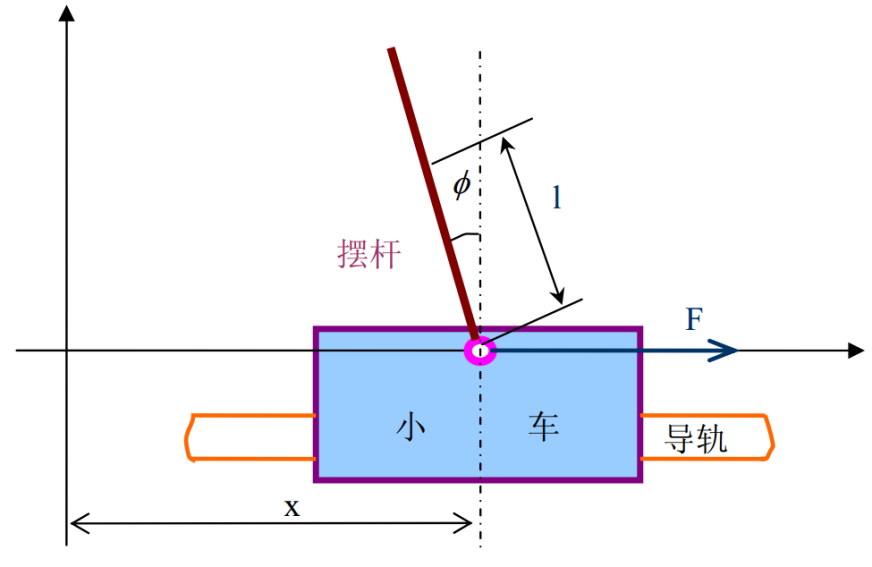
\includegraphics[width=0.6\textwidth]{model}\\
	\caption{简化模型}\label{model}
\end{figure}

插入双栏图片:图片名+图片标题+图片标签,如图\ref{step},\ref{sin}所示:
\dpicl{model}{阶跃干扰信号}{step}{model}{正弦干扰信号}{sin}

\subsection{问题提出}


    \section{问题分析}

    \section{问题一} 
    \section{问题二}
    \section{问题三}
    \section{模型分析与评估}

    \begin{thebibliography}{0}

\bibitem{jixie}
陈秀宁,顾大强.机械设计.浙江大学出版社,2010

\bibitem{tuxue}
谭建荣,张树有,陆国栋,施岳定编. 图学基础教程. 北京:高等教育出版社,2006
\end{thebibliography}
    \newpage
\section*{附录}

\begin{lstlisting}[language=matlab]      %%其中为matlab代码
    %%%100points
    clear all;clc;
    Fs = 10;                 % Sampling frequency
    T = 1/Fs;                % Sample time
    L = 100;                 % Length of signal 100
    t = (0:L-1)*T;           % Time vector
    % Generate the signal
    x=2.6*sin(4.2*pi*t+unifrnd(0,4*pi));
    y=2.1*sin(4.4*pi*t+unifrnd(-pi,pi));
\end{lstlisting}
    
\end{document}